%author: Pedro Pinto; v3; july 2020
\documentclass[11pt,a4paper]{report}
\usepackage[utf8]{inputenc}
\usepackage{amsmath}
\usepackage{graphicx}
\usepackage{tabularx}
\usepackage[spanish]{babel}
\usepackage{adjustbox}
%\usepackage[colorinlistoftodos]{todonotes}
\usepackage{lipsum}
\usepackage{csquotes}
\usepackage{comment}
\usepackage{imakeidx}
%tabela
\usepackage{multirow}
\usepackage{xcolor}
\usepackage[margin=3cm]{geometry}
\usepackage[hidelinks]{hyperref}
\usepackage[toc,acronym,nopostdot,nonumberlist]{glossaries}
\usepackage{titling}
\usepackage{tikzpagenodes}
\usepackage[ddmmyyyy]{datetime}
\usepackage{setspace}
\usepackage{indentfirst}
\selectlanguage{spanish}
\usepackage{float}
\usepackage{titlesec}

%para definir a localização das tabelas e imagens em modo strict
%\usepackage{placeins}

\usepackage{biblatex}
\addbibresource{ref.bib}
\doublespacing

\begin{document}
\pagenumbering{roman}
\begin{titlepage}
\begin{tikzpicture}[remember picture,overlay,shift={(current page.center)}]
\node[anchor=center,yshift=9cm]{
\includegraphics[scale=0.2]{figs/logo_utn.png}};
\end{tikzpicture}

\titleformat{\subsection}[runin]{}{}{}{}[]

\centering
\vspace{7cm}
\huge Informe de la práctica de laboratorio \#1 realizado para la materia Teoría de Circuitos 2\\
\vspace{2cm}


\Large Bruno Glecer\\
\vspace{2cm}
\large Materia dictada por\\
\large Mariano Llamedo Soria\\
\vspace{2cm}
\newdateformat{daymonthyear}{\THEDAY\ \monthname[\THEMONTH], \THEYEAR}
\daymonthyear\today \\
\vspace{1cm}
%December, 2019
%\large v2.3
\end{titlepage}



%%%%%%%%%%%%%%%%%%%%%%%%%%%%%%%%%%%%%%%%%%%%%%%%%%%%%  
\chapter*{\centering\Large\bfseries Introducción}

Este informe trata de la practica de laboratorio realizado el 22 de Junio de 2023 para la materia Teoria de Circuitos II en el curso R4001 dictada por Mariano Llamedo en la Facultad Regional de Buenos Aires de la Universidad Tecnológica Nacional. La preparación y realización del laboratorio fue realizada por el equipo constituido por: Bruno Glecer (autor del informe), Santiago Palozzo y Axel Nahum. Este trabajo tuvo la finalidad de llevar a la práctica la mayoría de los temas enseñados durante el primer cuatrimestre. Mas específicamente, se utilizaron los métodos modernos de aproximación de funciones de filtrado incluyendo transformaciones en frecuencia y la implementación de filtros activos utilizando amplificadores operacionales.

\tableofcontents

%%%%%%%%%%%%%%%%%%%%%%%%%%%%%%%%%%%%%%%%%%%%%%%%%%%%%  


\chapter{Desarrollo Matematico}
\section{Consigna} 

\pagenumbering{arabic}

El objetivo de este trabajo práctico consiste en el diseño, análisis, medición y discusión de un filtro activo. Este filtro debía ser implementado utilizando el circuito integrado UAF42 \cite{uaf42}. Este consiste de cuatro amplificadores operacionales y dos capacitores de alta precisión integrados de tal forma que hace sencillo diseñar cualquier filtro de orden dos e incluso algunos de orden tres solamente usando resistencias externas.

Nuestro equipo fue dada la tarea de realizar un filtro con las siguientes características:

\begin{itemize}
  \item Filtro pasa banda con aproximación Chebyshev
  \item Frecuencia central en $f_0=6 \mathrm{kHz}$
  \item Factor Q del filtro igual a 3
  \item Atenuación máxima en la banda de paso de $\alpha_{max} = 2.5 \mathrm{dB}$
  \item Extremos de la banda inferior y superior de stop de $f_{s1} = 600 \mathrm{Hz}$ y $f_{s2} = 60 \mathrm{kHz}$ respectivamente
  \item Atenuación mínima en los extremos de las bandas de stop de $\alpha_{min} = 15 \mathrm{dB}$
\end{itemize}

\section{Calculos preliminares}

Comenzamos el diseño del filtro calculando algunos parámetros adicionales útiles:

\begin{itemize}
    \item Ancho de banda: $\mathrm{BW} = \dfrac{f_0}{Q} = 2\mathrm{kHz}$
    \item Banda de paso: $f_{p1} = 7.0828\mathrm{kHz}$  \hspace{10pt} a \hspace{10pt} $f_{p2} = 5.0828\mathrm{kHz}$
\end{itemize}

La banda de paso fue encontrada utilizando: $f_0 = \sqrt{f_{p1} f_{p2}}$ \hspace{5pt} y \hspace{5pt} $\mathrm{BW} = f_{p2} - f_{p1}$

Esto nos permite obtener una plantilla gráfica del filtro para mayor claridad de las características.
\vspace{1cm}


\begin{figure}[h]
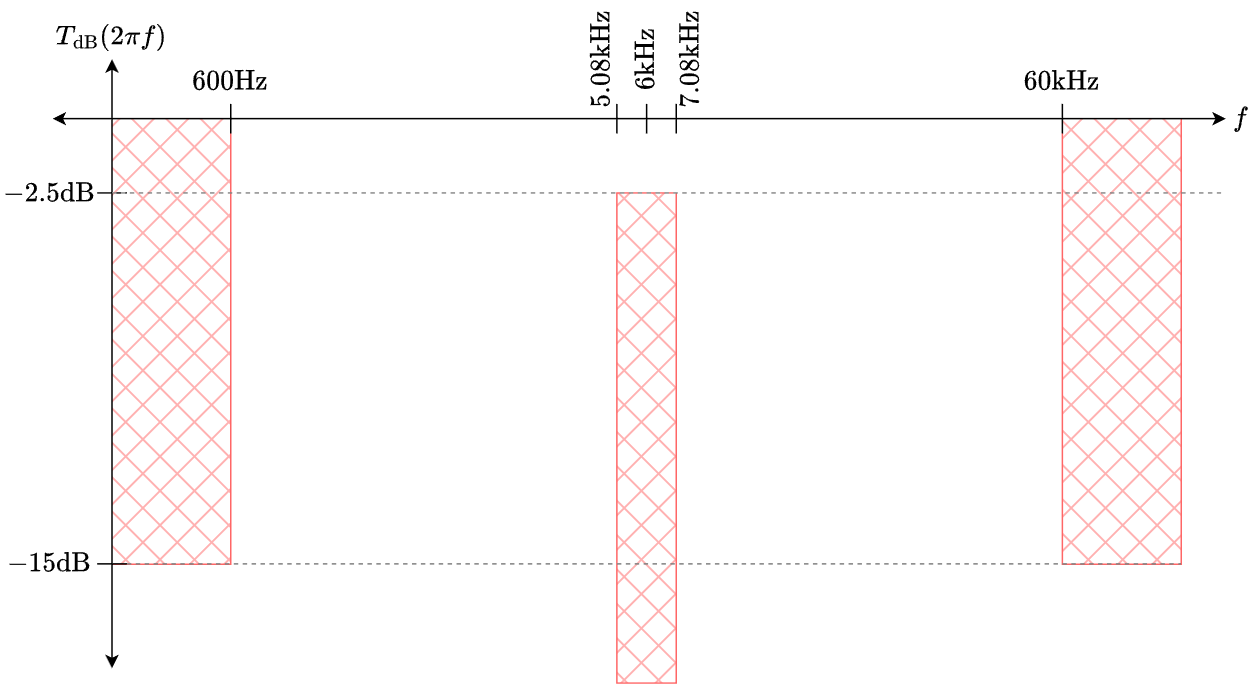
\includegraphics[scale=0.45]{figs/plantilla.png}
\caption{Plantilla del filtro objetivo}
\end{figure}


\section{Normalización}

Como toda situación en la que se implementa un filtro utilizando la teoría moderna, es conveniente trabajar utilizando frecuencias normalizadas. Para esto, tomamos una frecuencia que usaremos como norma, en el caso de un pasa banda, la frecuencia que se suele tomar es la frecuencia central.
De este punto en adelante todas las frecuencias expresados en forma de frecuencia angular utilizando la letra $\omega$, estarán normalizadas entorno a $2 \pi f_0$. Esto nos deja con los siguientes parámetros de diseño:

\begin{itemize}
    \item $\omega_0 = 1$ (por definición de la norma)
    \item $\omega_{p1} = 0.84713$ \hspace{5pt} $\omega_{p2} = 1.1805$
    \item $\omega_{s1} = 0.1$ \hspace{5pt} $\omega_{s2} = 10$

\end{itemize}

\section{Planteo del filtro prototipo}

Para encontrar la transferencia que satisfaga las condiciones de la plantilla pedida, primero diseñaremos un filtro prototipo. Este será un filtro pasa-bajos, del cual usaremos su función de transferencia $T_{LP}(p)$, para transformarla a la de un filtro pasa banda $T(s)$. La transformación se realiza sustituyendo la variable de frecuencia compleja $p = \Sigma + j\Omega$ por una función en términos de la variable $s$. Esta función se la denomina el núcleo de transformación.

Para transformar de un pasa bajos a un pasa banda resulta muy útil el núcleo: \newline
$$p = K(S) = Q \dfrac{s^2 + 1}{s}$$

Este tiene la propiedad de mapear $p=\pm j$ a las frecuencias de corte $s=\pm j\omega_{p1}$ y $s=\pm j\omega_{p2}$, y de mapear $p=0$ a la frecuencia central $s=\pm j$.
Diseñando un pasa bajos con una cierta atenuación $\alpha$ en $p = \pm j$ y transformándolo usando este núcleo, resultará en un filtro pasa banda con frecuencia central $\omega = 1$, ancho de banda normalizado $\dfrac{1}{Q}$ y atenuación $\alpha$ en las frecuencias de corte. Este filtro siempre resulta ser simétrico respecto de $\omega_0$ (visto en una escala de frecuencias logarítmicas).

Dicho esto, comenzamos diseñado el filtro pasa bajos. Para esto tenemos que elegir cuidadosamente sus parámetros de diseño. Empezamos por su frecuencia de corte:

La frecuencia de corte tiene que ser elegida para que cuando se diseñe y se transforme a una transferencia pasa banda, cumpla con la plantilla original. Para esto la frecuencia de corte del prototipo debe ser elegida para que le imponga la mayor exigencia al diseño, de esta forma cuando se transforme al filtro pasa banda aseguramos de que ambas pendientes de roll-off estén dentro de los parámetros exigidos en la plantilla.

Transformando ambas frecuencias de los extremos de la banda de corte, obtenemos:

\begin{itemize}
    \item $|K(j \omega_s1)| = 29.7$
    \item $|K(j \omega_s2)| = 29.7$
\end{itemize}

Ambas opciones son idénticas, esto es de esperar ya que ambas frecuencias de la banda de corte están a la misma distancia (logaritmica) de la frecuencia central $\left( \dfrac{600Hz}{6kHz} = \dfrac{6kHz}{60kHz} \right)$.


Buscamos entonces diseñar primero un filtro pasa bajos con atenuación $\alpha_{max} = 2.5 \mathrm{dB}$ en la frecuencia de corte $\Omega = 1$ y una atenuación mínima de $\alpha_{min} = 15 \mathrm{dB}$ en la frecuencia de corte $\Omega = 29.7$.

Al ser un filtro de aproximación Chebyshev, sabemos que la función de transferencia de potencia tendrá la siguiente forma:

$$|T_{LP}(j\Omega)|^2 = \dfrac{1}{1 + \varepsilon^2 C_n^2(\Omega)}$$

Donde $C_n(\Omega)$ es el enésimo polinomio de aproximación de Chebyshev de primer tipo y $\varepsilon$ es un parámetro que define la atenuación en la frecuencia de corte. Si $\varepsilon = 1$ la atenuación en la frecuencia de corte será de aproximadamente $3\mathrm{dB}$, un valor estándar.

Empezamos calculando el parámetro $\varepsilon$, este se puede calcular fácilmente con la siguiente expresión derivada de la expresión genérica de la función de transferencia y la definición de atenuación:

$$\varepsilon = \sqrt{10^{\dfrac{\alpha_{max}}{10}} - 1} \approx 0.8222 $$

Continuamos calculando el orden que requiere el filtro para lograr la atenuación en la banda de corte. Esto se puede lograr iterando valores de $n$ comenzando en $n=1$ hasta encontrar el orden mínimo que cumpla la condición de diseño. Una formula útil para los polinomios de Chebyshev para $x>1$ es: $C_n(x) = cosh(n ~ cosh^{-1} (x)) $

La formula cerrada de la atenuación (para $\Omega > 1$) resulta:

$$\alpha_{LP}(\Omega) = 10 ~ log(1 + \varepsilon^2 (cosh(n ~ cosh^{-1} (\Omega)))^2)$$

Partiendo de $n=1$ ya encontramos que este valor alcanza la atenuación requerida en $\Omega_s$ de $15\mathrm{dB}$

$$10 ~ log(1 + \varepsilon^2 (cosh(1 ~ cosh^{-1} (\Omega_s)))^2) = 28.37\mathrm{dB}$$

Concluimos que el orden mínimo del filtro prototipo resulta ser de $n = 1$.

Continuamos encontrando la expresión racional de la función de transferencia. Para esto identificamos el polinomio de Cebyshev $C_1(x)$, este es: $C_1(x) = x$. Remplazando en la expresión de $T_{LP}(j\Omega)$ obtenemos:

$$|T_{LP}(j\Omega)|^2 = \dfrac{1}{1 + \varepsilon^2 \Omega^2}$$

Remplazando $j\Omega$ por su expresión mas general $\Omega = \dfrac{p}{j}$

$$|T_{LP}(p)|^2 = \dfrac{1}{1 + \varepsilon^2 \left(\dfrac{p}{j}\right)^2} = \dfrac{1}{1 - \varepsilon^2 p^2} = \dfrac{-\varepsilon^{-2}}{p^2 - {\varepsilon^{-2}}}$$

Para obtener $T_{LP}(p)$ utilizamos la relación $|T_{LP}(p)|^2 = T_{LP}(p) T_{LP}(-p)$. Es importante que $T_{LP}(p)$ se defina de forma tal que todos los polos se encuentren en el semiplano izquierdo para que el filtro sea estable.

$$
\dfrac{-\varepsilon^{-2}}{p^2 - {\varepsilon^{-2}}} =
\underbrace{\dfrac{\varepsilon^{-1}}{p + \varepsilon^{-1}}}_{T_{LP}(p)}
\underbrace{\dfrac{\varepsilon^{-1}}{(-p) + \varepsilon^{-1}}}_{T_{LP}(-p)}
$$

$$T_{LP}(p) = \dfrac{\varepsilon^{-1}}{p + \varepsilon^{-1}}$$

\section{Transformación a basa banda}

Ahora podemos substituir $p = K(s) = Q \dfrac{s^2 + 1}{s}$ en $T_{LP}$:

$$T(s) = \dfrac{\varepsilon^{-1}}{Q \dfrac{s^2 + 1}{s} + \varepsilon^{-1}} $$
$$T(s) = \dfrac{\varepsilon^{-1}s}{Q (s^2 + 1) + \varepsilon^{-1}s} $$
$$T(s) = \dfrac{(Q \varepsilon)^{-1}s}{s^2 +  (Q \varepsilon)^{-1}s + 1} \approx \dfrac{0.3778s}{s^2 +  0.3778s + 1}$$

Así finaliza el desarrollo matemático de la función de transferencia del filtro que la consigna pide.

\section{Implementación Circuital}

Para implementar el filtro no utilizaremos amplificadores operacionales discretos. Estos tienen la desventaja de que es necesario utilizar algun componente reactivo externo. Estos suelen tener tolerancias muy altas, en el orden del 10\% comparado con resistencias que se obtienen facilmente de 1\%. Para superar este problema, utilizaremos el UAF42\cite{uaf42} de Texas Instruments. El diseño interno de este dispositivo es el siguiente:

\begin{figure}[h]
\centering
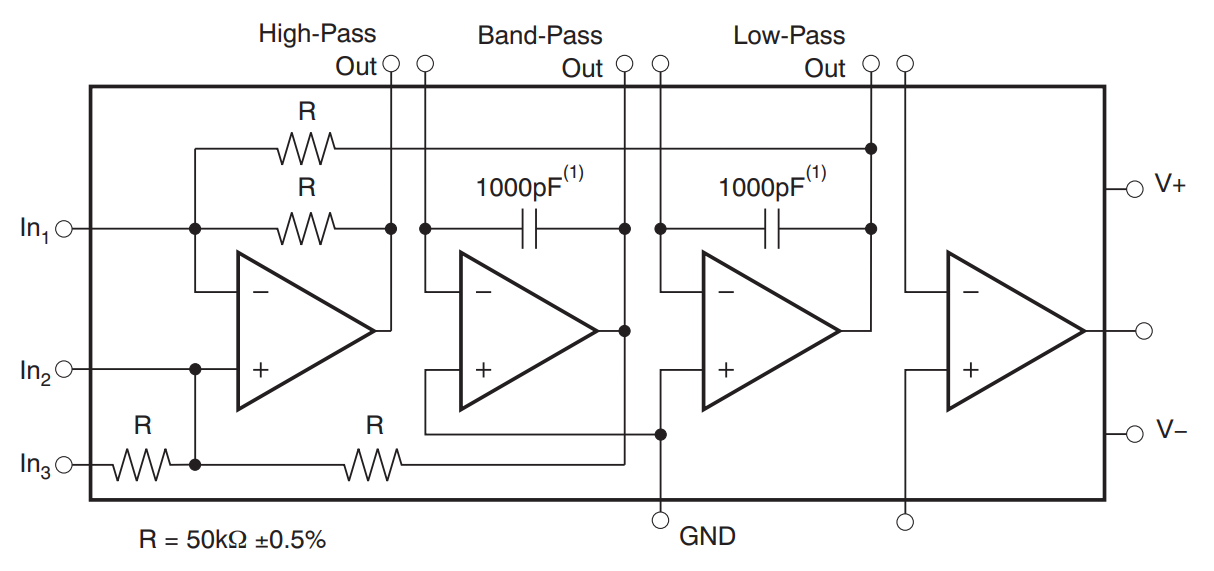
\includegraphics[scale=0.35]{figs/uaf42_internals.png}
\caption{Interior del UAF42}
\end{figure}

El datasheet nos da propuestas de uso para distintos tipos de filtros. El circuito que el datasheet propone para un no inversor es:

\begin{figure}[h]
\centering
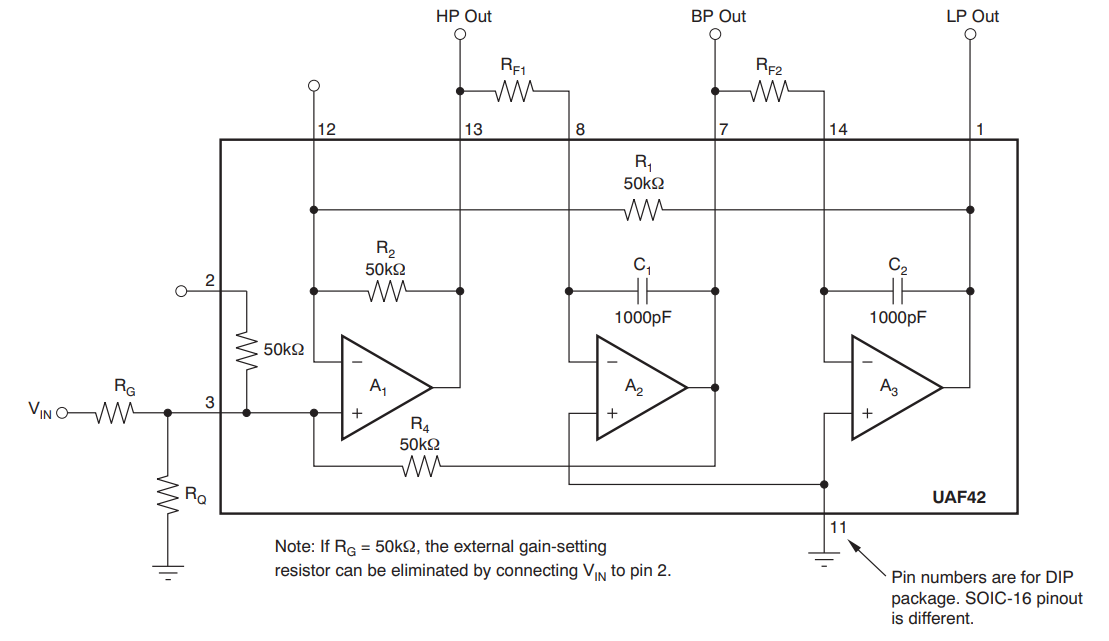
\includegraphics[scale=0.5]{figs/uaf42_non_inv.png}
\caption{Uso del UAF42 en modo no inversor}
\end{figure}

También nos provee con formulas útiles para obtener los valores de los componentes.

\begin{figure}[h]
\label{uaf42_eq}
\centering
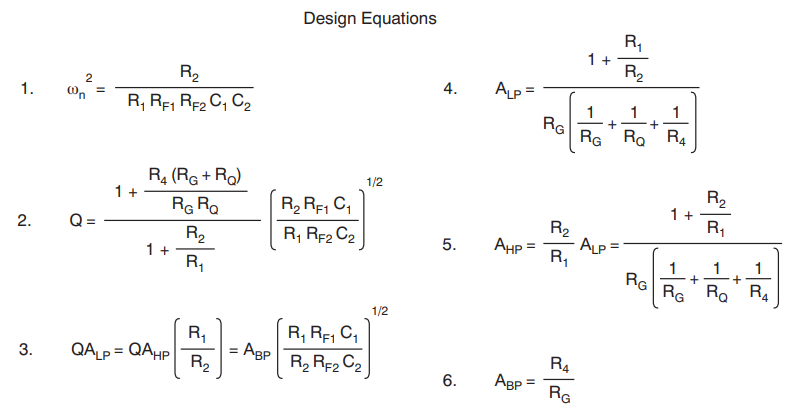
\includegraphics[scale=0.6]{figs/uaf42_eq.png}
\caption{Ecuaciones de diseño}
\end{figure}

Como estaremos saliendo por la salida pasa banda, las ecuaciones que mas nos interesan son: 1, 2 y 6.
Y la transferencia del filtro expresada en términos de estos parámetros según el datasheet es:

$$T(s) = A_{BP} \dfrac{ \dfrac{\omega_0}{Q_p} s}{s^2 + \dfrac{\omega_0}{Q_p}s + 1}$$

Es importante notar que $Q_p$ no es lo mismo que $Q$. La primera es el factor Q de los polos del sistema $\left( Q_p = \dfrac{1}{2 cos(\varphi)} \right)$, mientras que la segunda es el factor Q del diseño del filtro pasa banda $\left( Q = \dfrac{f_0}{BW} \right)$. Para el caso del filtro que estamos diseñando, la relación entre ellas es: $Q_p = Q \varepsilon$


Como muestra el datasheet, las resistencias $R_1$, $R_2$ y $R_4$ son de $50k\Omega$ y $C_1$ y $C_2$ son de $1nF$. 

Recordemos la función de transferencia que deseamos implementar:

$$T(s) = \dfrac{0.3778s}{s^2 +  0.3778s + 1}$$

Primero observamos que $A_{BP} = 1$. Esto, junto con la ecuación 6 de la figura \ref{uaf42_eq} nos lleva a que la resistencia externa $R_G$ es de $50k\Omega$. Convenientemente, el dispositivo tiene una resistencia integrada de $50k\Omega$ que se puede usar para este propósito si la señal de entrada se aplica en el pin 2.

Para determinar el resto de los componentes hay que fijar un valor para alguno de ellos. Elegimos fijar la resistencia $R_{F1}$ a $10k\Omega$ y dejar que el resto de los valores se determinen a partir de esa elección.

El valor deseado para la frecuencia central es de $\omega_0 = 2 \pi ~ 6\mathrm{kHz} \approx 37.7 \mathrm{k ~ s^{-1}}$.

Utilizando la ecuación 1 de la figura \ref{uaf42_eq} podemos llegar a:

$$R_{F2} = \dfrac{1}{\omega_0^2 R_{F1} C_1^2} \approx 70.36k\Omega$$

Y utilizando la ecuación 2, llegamos a:

$$R_Q = \dfrac{R}{2Q_p\sqrt{\dfrac{R_{F2}}{R_{F1}}} - 2} \approx 4.153 k\Omega$$

Para fabricar este circuito necesitamos utilizar valores comerciales, idealmente de la serie E12. Para obtener mayor precisión, las resistencias que no tienen valores exactos ($R_{F2}$ y $R_Q$) fueron elegidas utilizando una herramienta online \cite{res_calc} que encuentra combinaciones de dos valores comerciales para aproximarse lo mas posible al valor deseado.

Los valores comerciales elegidos fueron:

\begin{itemize}
    \item $R_{F1} = 10 k\Omega$ (exacto)
    \item $R_{F2} = 68k\Omega + 2.2k\Omega = 70.2k\Omega$  (-0.2\% diferencia)
    \item $R_Q = 3.9k\Omega + 270\Omega = 4.17k\Omega$  (+0.4\% diferencia)
\end{itemize}

Así concluimos el trabajo de diseño del filtro

\chapter{Simulación}

\section{Esquemático}

Para la simulación numérica del circuito, utilizamos el software de simulación LTSpice.
A continuación se muestra el esquemático de la simulación realizada

\begin{figure}[h]
\centering
\label{sim_sch}
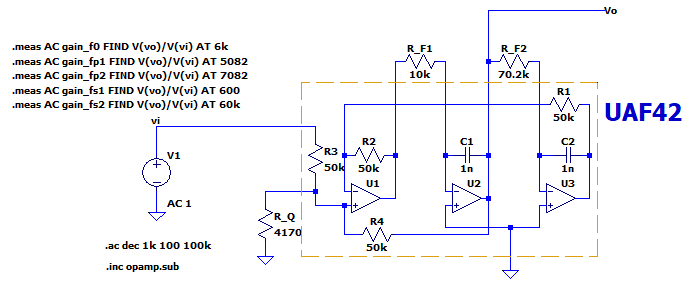
\includegraphics[scale=0.8]{figs/sim_sch.png}
\caption{Esquematico de la simulación en LTSpice}
\end{figure}

El modelo del amplificador utilizado es el modelo opamp.sub incluido en LTSpice.

\section{Resultados}


La respuesta de la ganancia y fase en función de la frecuencia fue la siguiente:

\begin{figure}[H]
\centering
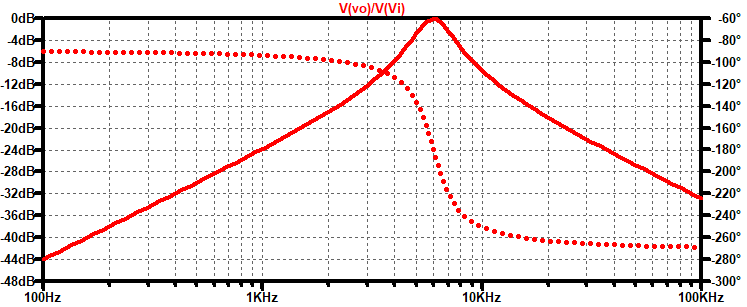
\includegraphics[scale=0.55]{figs/sim_plt.png}
\caption{Resultado de simulación - Respuesta en frecuencia}
\end{figure}

Y los resultados de las mediciones de ganancia:

\begin{table}[H]
    \centering
    \begin{tabular}{c|c|c}
    Frecuencia & Ganancia esperada & Ganancia medida en simulación\\
    \hline
    $f_0$: 6kHz         & 0dB & 0.001dB \\
    \hline
    $f_{p1}$: 5.08kHz   & -2.5dB & -2.52dB \\
    \hline
    $f_{p2}$: 7.08kHz   & -2.5dB & -2.46dB \\
    \hline
    $f_{s1}$: 600Hz     & -28.4dB & -28.4dB \\
    \hline
    $f_{s2}$: 60kHz     & -28.4dB & -28.3dB \\
    \end{tabular}
    \caption{Resultado se simulación - Mediciones en frecuencias criticas}
    \label{tab:my_label}
\end{table}

Estos valores confirman que el filtro se encuentra bien diseñado y podemos continuar a la etapa de implementación física.

\chapter{Construcción}

El circuito que armamos para el día del laboratorio es el mismo circuito que se simuló en LTSpice como se muestra en la figura \ref{sim_sch}.

Las única diferencia fue el uso de capacitores de filtrado conectados en las entradas de alimentación del UAF42.

\begin{figure}[h]
\centering
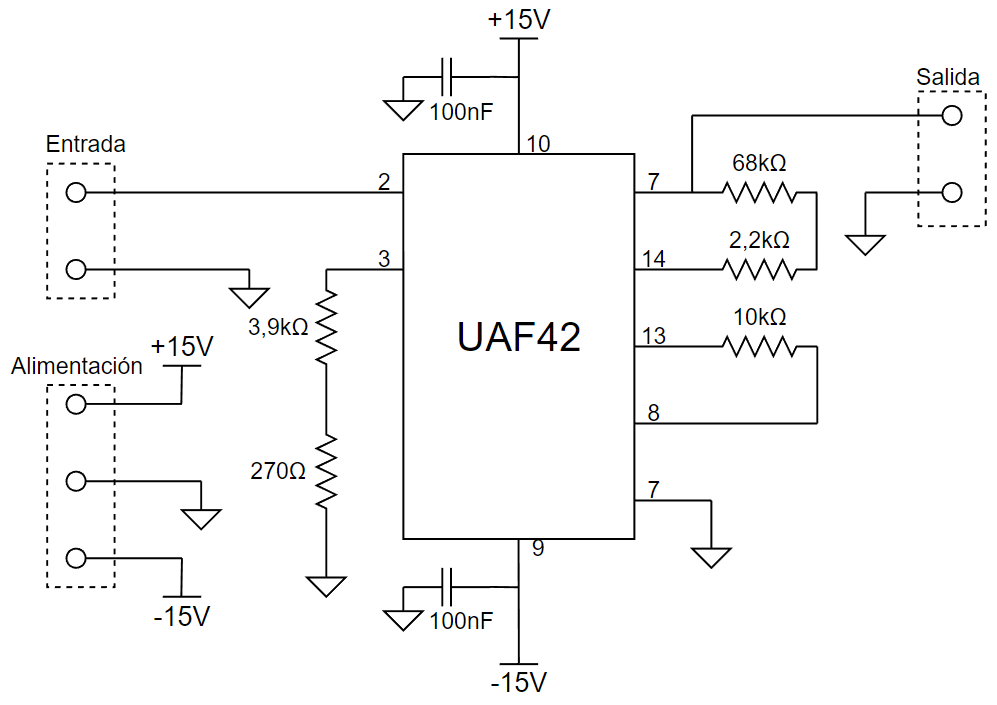
\includegraphics[scale=0.5]{figs/pcb_sch.png}
\caption{Esquematico de la implementación del filtro}
\end{figure}

Para el armado, al ser un circuito relativamente sencillo, de pocos componentes y ninguno de montaje superficial, optamos por utilizar una placa universal en lugar de desarrollar nuestro propio PCB. Afortunadamente, encontramos todos los componentes necesarios en el pañol del departamento de electrónica.
Los componentes utilizados fueron los siguientes:

\begin{itemize}
    \singlespacing
    \item 1  Placa universal especifica para circuitos con ICs DIP.
    \item 1  Filtro activo universal UAF42
    \item 1  Zócalo DIP-14
    \item 2  Capacitores 100nF cerámicos
    \item 1  Resistencia 10k$\Omega$ $\pm$ 5\%
    \item 1  Resistencia 10k$\Omega$ $\pm$ 5 \%
    \item 1  Resistencia 3,9k$\Omega$ $\pm$ 5\%
    \item 1  Resistencia 270$\Omega$ $\pm$ 5\%
    \item 1  Resistencia 2,2k$\Omega$ $\pm$ 5\%
    \item 1  Resistencia 68k$\Omega$ $\pm$ 5\%
\end{itemize}

A continuación se muestran imágenes de la placa finalizada:

\begin{figure}[h]
    \centering
    \begin{minipage}{0.45\textwidth}
\centering
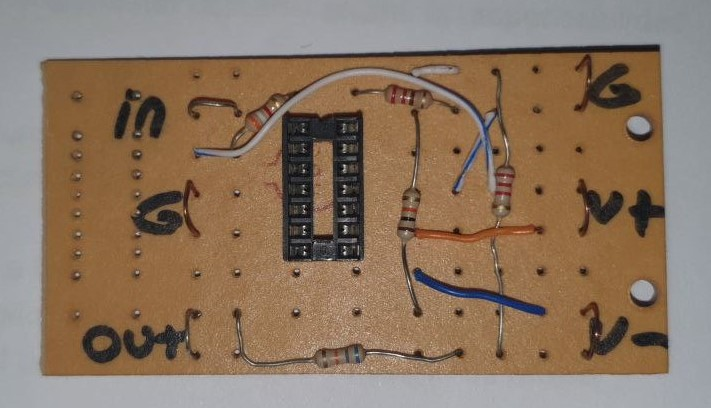
\includegraphics[scale=0.30]{figs/pcb_1.jpg}
\caption{Circuito finalizado - Vista superior}
    \end{minipage}\hfill
    \begin{minipage}{0.45\textwidth}
\centering
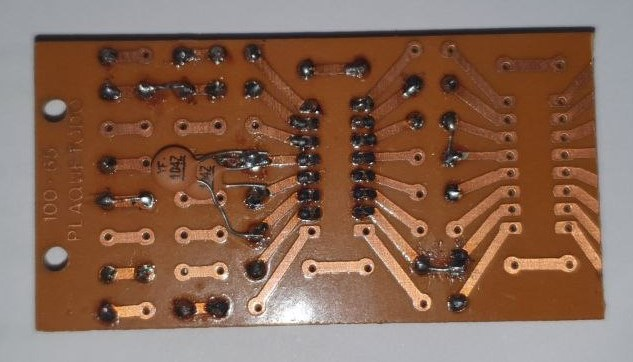
\includegraphics[scale=0.32]{figs/pcb_2.jpg}
\caption{Circuito finalizado - vista inferior}
    \end{minipage}
\end{figure}

\chapter{Mediciones en laboratorio}

El día del laboratorio, utilizamos una fuente de laboratorio partida para generar la tensión de alimentación del filtro, utilizamos cables de conector banana a cocodrilo para conectarla con la placa. También utilizamos un generador de funciones para producir la señal senoidal que se aplicó en la entrada utilizando un cable BNC a pares de cocodrilo.
Para las mediciones utilizamos un osciloscopio digital para visualizar y medir la señal de salida, para esto utilizamos una punta de osciloscopio estándar en modo X10.

\begin{figure}[h]
\centering
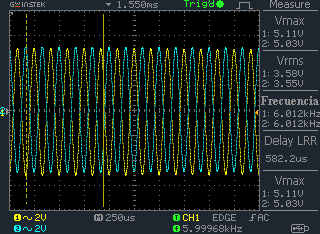
\includegraphics[scale=1]{figs/osc_f0.png}
\caption{Lectura del osciloscopio en la frecuencia central}
\end{figure}

La tensión de entrada fue elegida para ser el valor mas alto sin que el filtro distorsione. Esto lo logramos comenzando con una tensión de entrada que distorsiona, luego utilizando la función FFT del osciloscopio para observar las harmónicas fuimos disminuyendo la tensión hasta que no se podían ver a simple vista las harmónicas de la señal. Esto ocurrió alrededor de los 3.6Vrms. Elegimos utilizar esta tensión de entrada para las mediciones.

Las amplitudes de entrada y salida fueron medidas utilizando la función de medición RMS del osciloscopio, este método tiene la ventaja de tener menos ruido que medir solamente los picos de la señal, ya que utiliza todos los puntos de la señal para producir esta medición.

Para realizar las mediciones temporales, utilizamos los cursores horizontales del osciloscopio, que fueron colocados por observación en los cruces por cero de las señales para medir el retardo de fase entre ellas.

Elegimos 31 valores de frecuencias distintas en donde realizar las mediciones, para cada una de estas frecuencias se midió: tensión de entrada, tensión de salida y retardo de fase.

Estos valores se encuentra en el archivo mediciones\_osciloscopio.csv del repositorio del informe \cite{val_osc_file}.

El segundo tipo de medición, se realizó utilizando un analizar de audio, un instrumento que tiene la capacidad de producir un barrido de frecuencias mientras mide la señal de salida, de donde puede muestrear la ganancia y la fase del filtro. Este se utilizo para medir estos dos parámetros entre las frecuencias de 60Hz a 60kHz. Los datos crudos de salida del instrumento se encuentran en mediciones\_analizador\_modulo.csv \cite{val_mag_analizador_file} y mediciones\_analizador\_fase.csv \cite{val_fase_analizador_file}



\chapter{Análisis y comparación}

Utilizando un script de Python, la librería pandas para leer los archivos CSV, numpy para procesar arrays de datos y matplotlib para realizar los gráficos podemos realizar una visualización y comparación de los distintos métodos de medición.
El código se encuentra subido al repositorio del informe \cite{notebook}.

\section{Respuesta de modulo}

\begin{figure}[H]
\centering
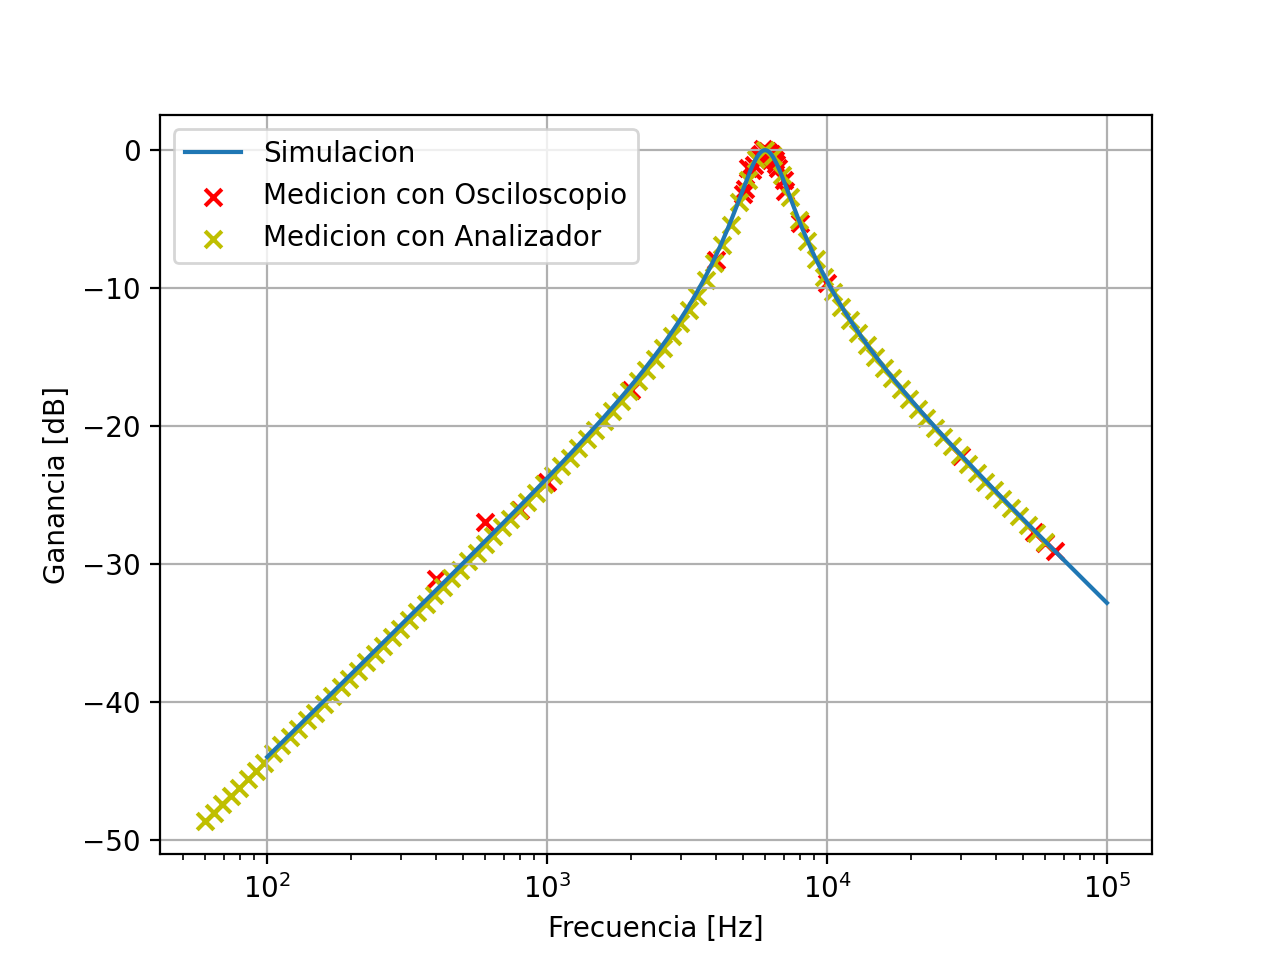
\includegraphics[scale=0.7]{figs/plots/mag.png}
\caption{Mediciones de respuesta de modulo}
\end{figure}

\begin{figure}[H]
\centering
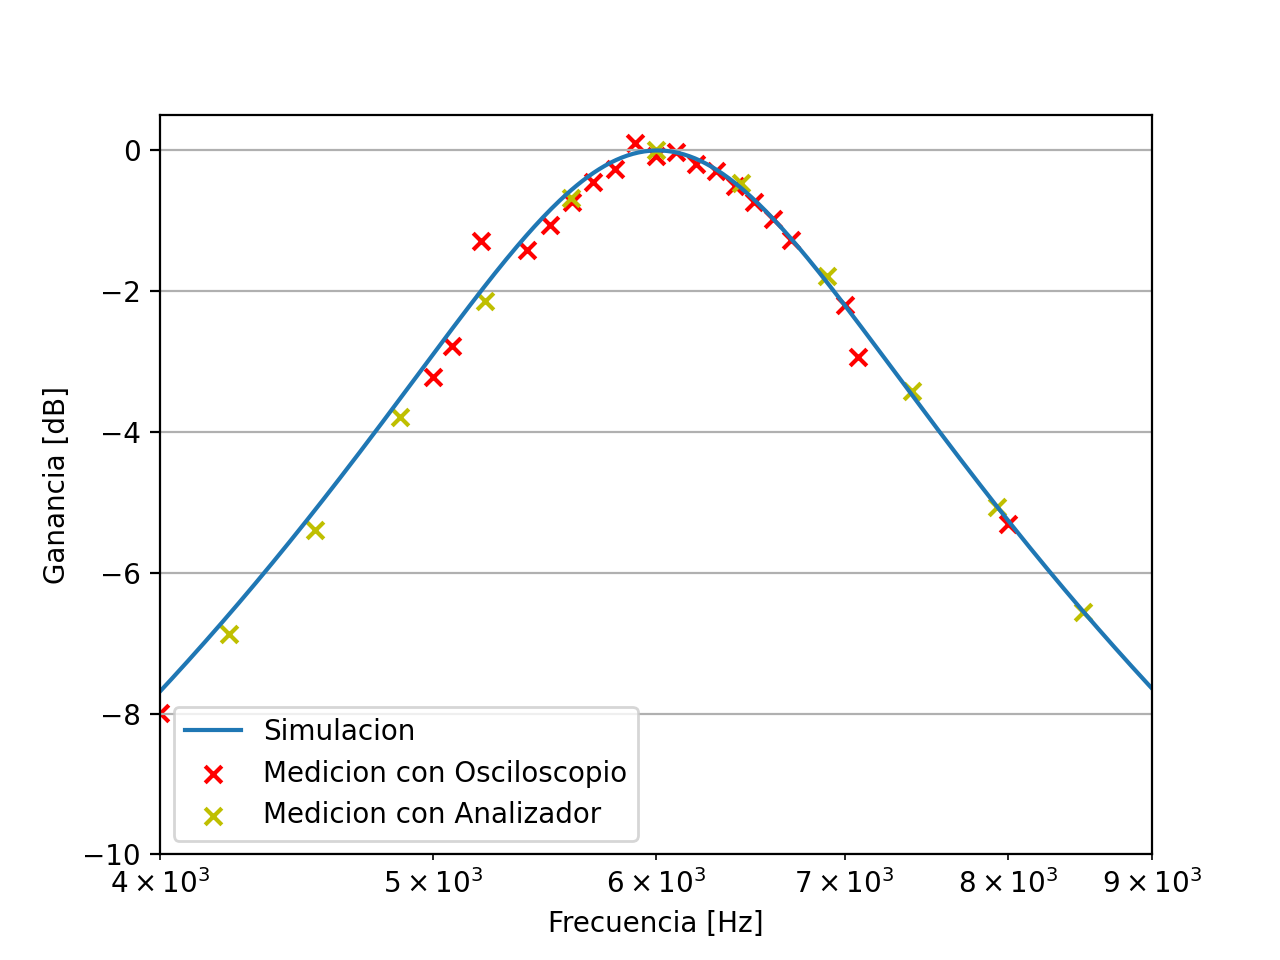
\includegraphics[scale=0.7]{figs/plots/mag_zoom.png}
\caption{Mediciones de respuesta de modulo cerca de la banda de paso}
\end{figure}

A simple observación se puede ver que el filtro se comporta muy similar a las predicciones teóricas. Aprovechamos para calcular la diferencia de cada medición con la esperada por la simulación.

\begin{figure}[h]
\centering
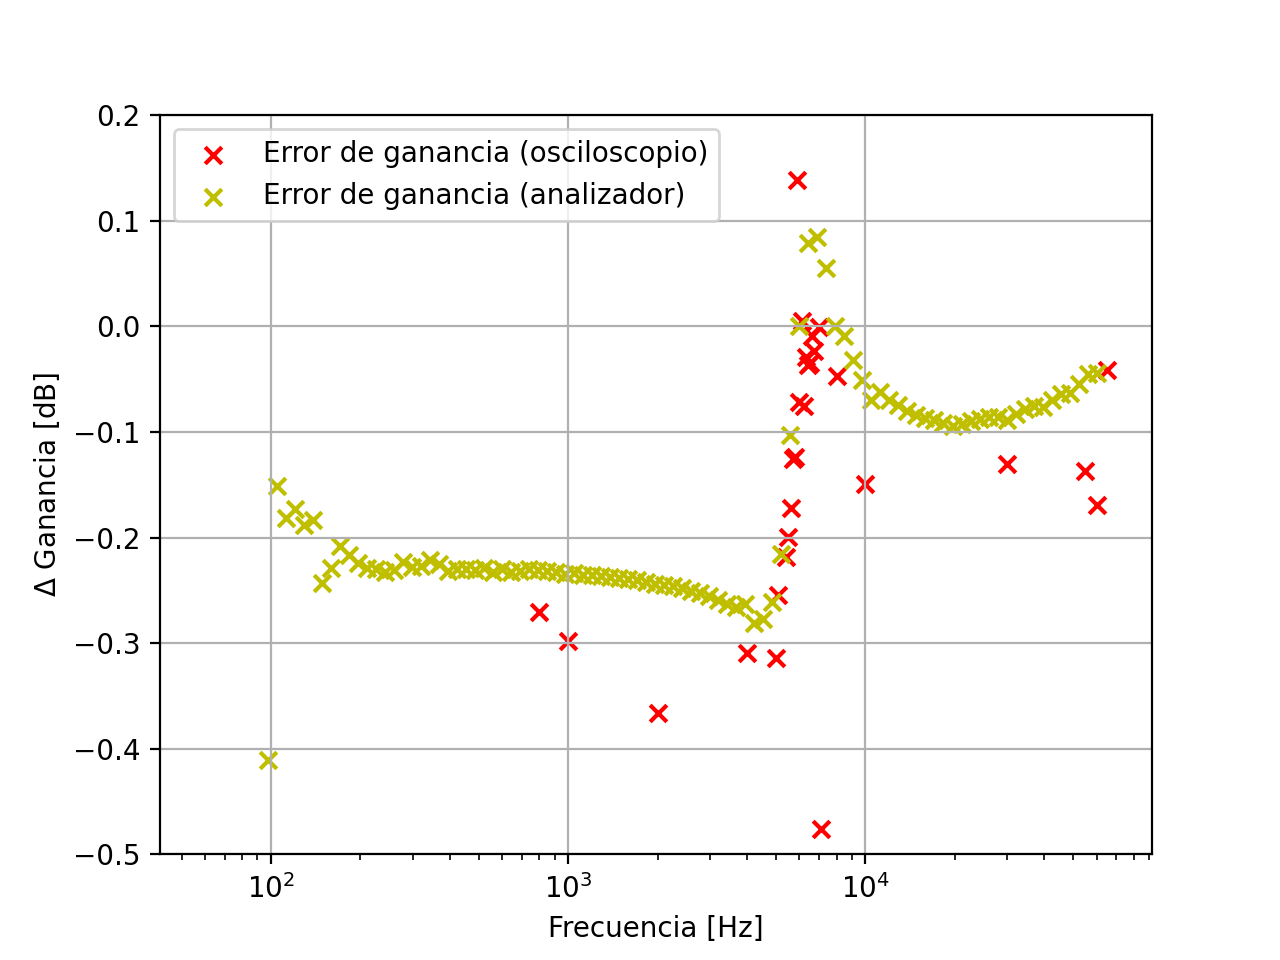
\includegraphics[scale=0.7]{figs/plots/mag_err.png}
\caption{Error de respuesta de modulo}
\end{figure}

Como se puede ver, la diferencia de ganancia para ninguno de los métodos supera 0.5dB. Podemos concluir entonces que el filtro se encuentra bien fabricado y los instrumentos lograron medir la respuesta de modulo con precisión.

\section{Respuesta de fase}

La respuesta de fase es un parámetro que solamente el analizador de audio mide directamente, el osciloscopio sin embargo mide el retardo de fase. Para calcular la respuesta de fase, utilizamos la siguiente relación que fue implementada en el script:

$$\phi = - \tau_{\phi} \omega$$

\begin{figure}[H]
\centering
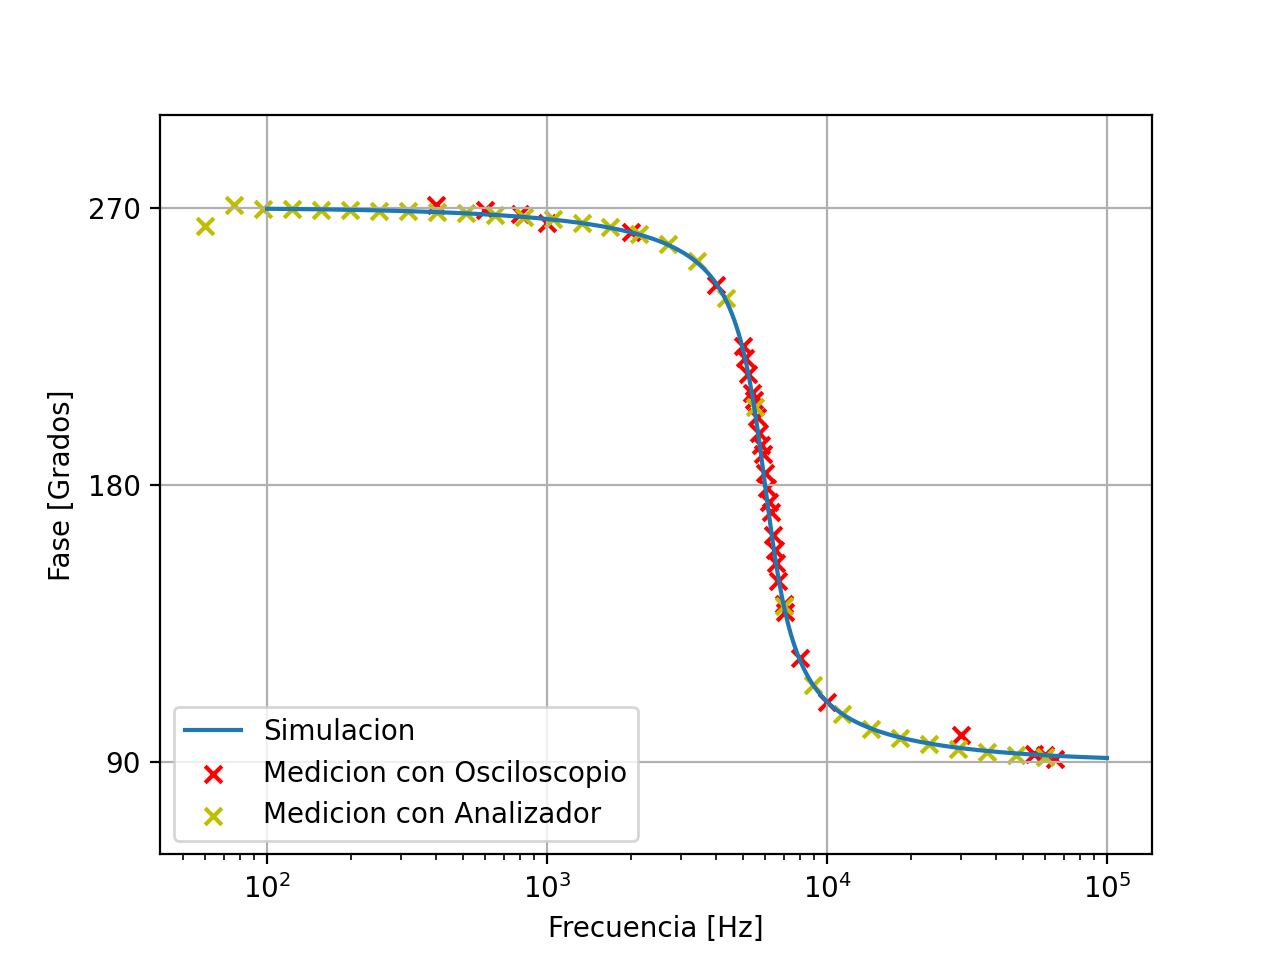
\includegraphics[scale=0.7]{figs/plots/fase.png}
\caption{Mediciones de respuesta de fase}
\end{figure}

\begin{figure}[H]
\centering
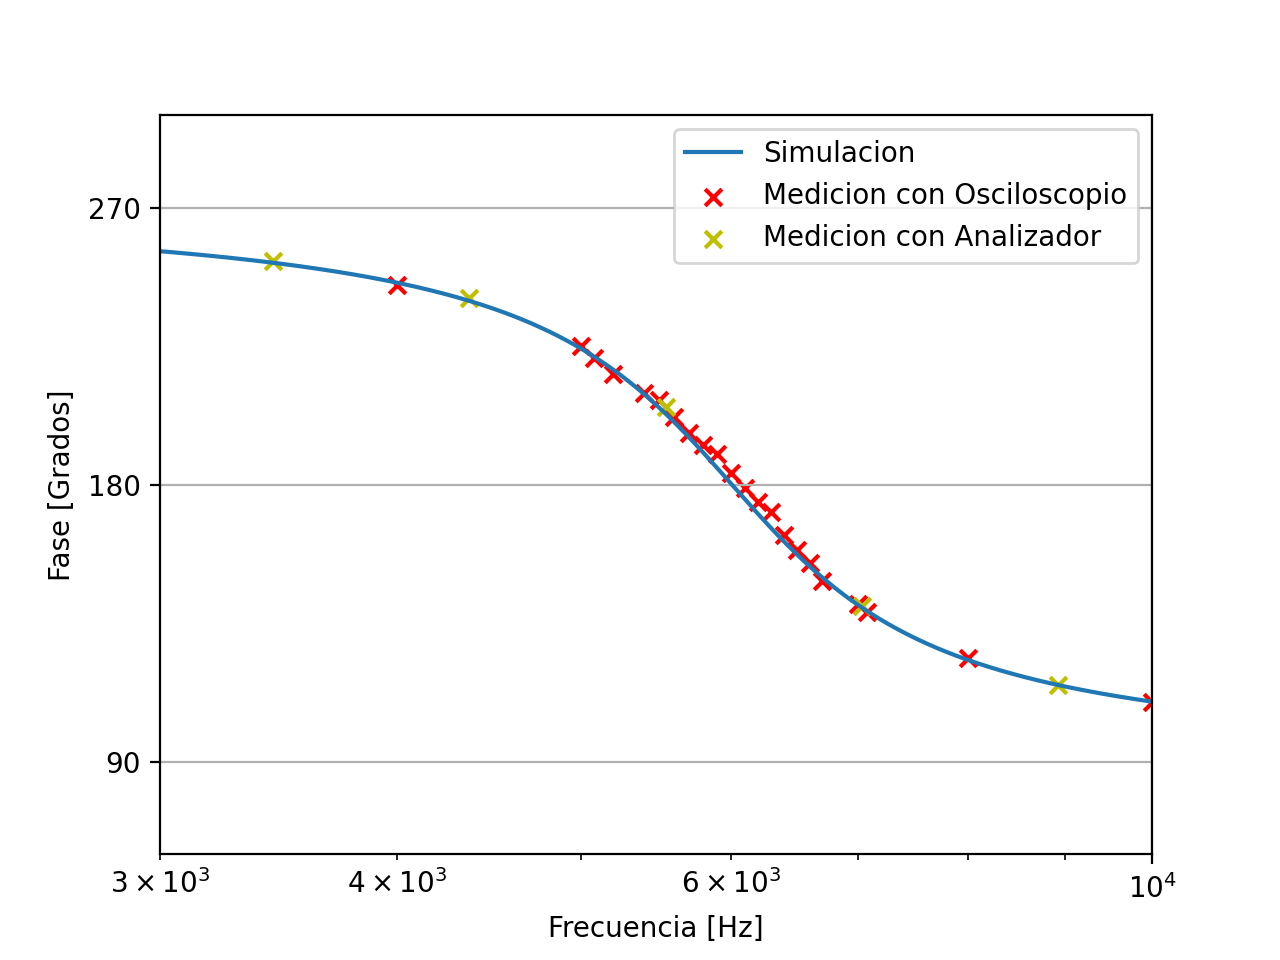
\includegraphics[scale=0.7]{figs/plots/fase_zoom.png}
\caption{Mediciones de respuesta de fase cerca de la banda de paso}
\end{figure}

Al igual que la respuesta de modulo, las mediciones de la respuesta de fase también produjeron valores muy cercanos a la teoría. Algo para notar es que las mediciones densas que decidimos tomar con el osciloscopio no cubren por completo la zona de transición de la fase, que es la parte mas interesante para analizar, esto se pudo haber evitado teniendo mejor criterio a la hora de elegir las frecuencias a medir.

\begin{figure}[H]
\centering
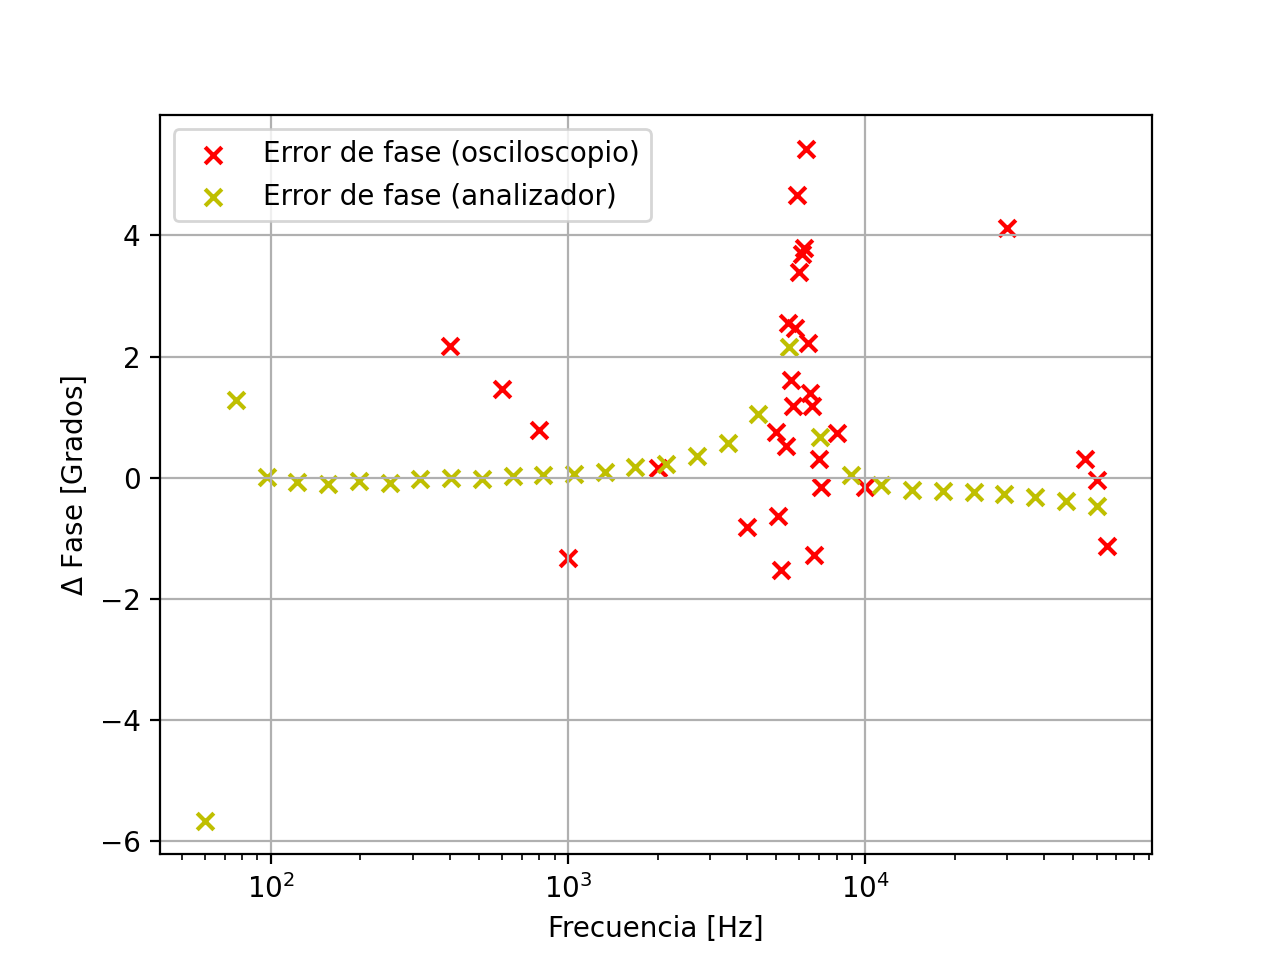
\includegraphics[scale=0.7]{figs/plots/fase_err.png}
\caption{Error de respuesta de fase}
\end{figure}


\section{Retardo de grupo}

El retardo de grupo no es algo que ninguno de los instrumentos mida directamente, para calcularlo utilizamos la siguiente relación:

$$\tau_{g}(\omega) = - \dfrac{d\phi}{d\omega}$$

O su versión discreta que fue implementada en el script:

$${\tau_g}_i = - \dfrac{ \phi_{i+1} - \phi_i }{ \omega_{i+1} - \omega_i }$$


\begin{figure}[H]
\centering
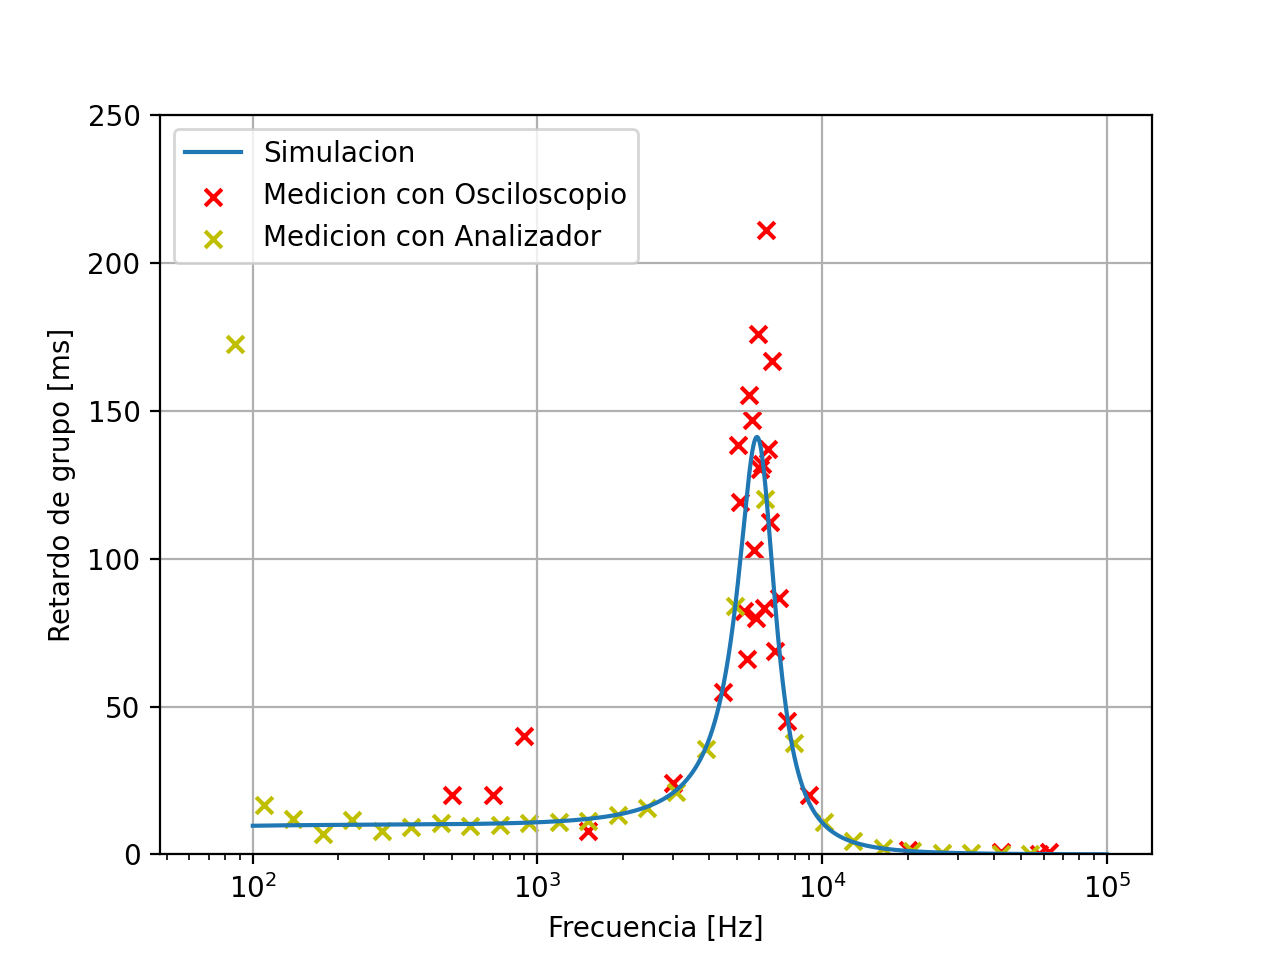
\includegraphics[scale=0.7]{figs/plots/delay.png}
\caption{Mediciones del retardo de grupo}
\end{figure}

\begin{figure}[H]
\centering
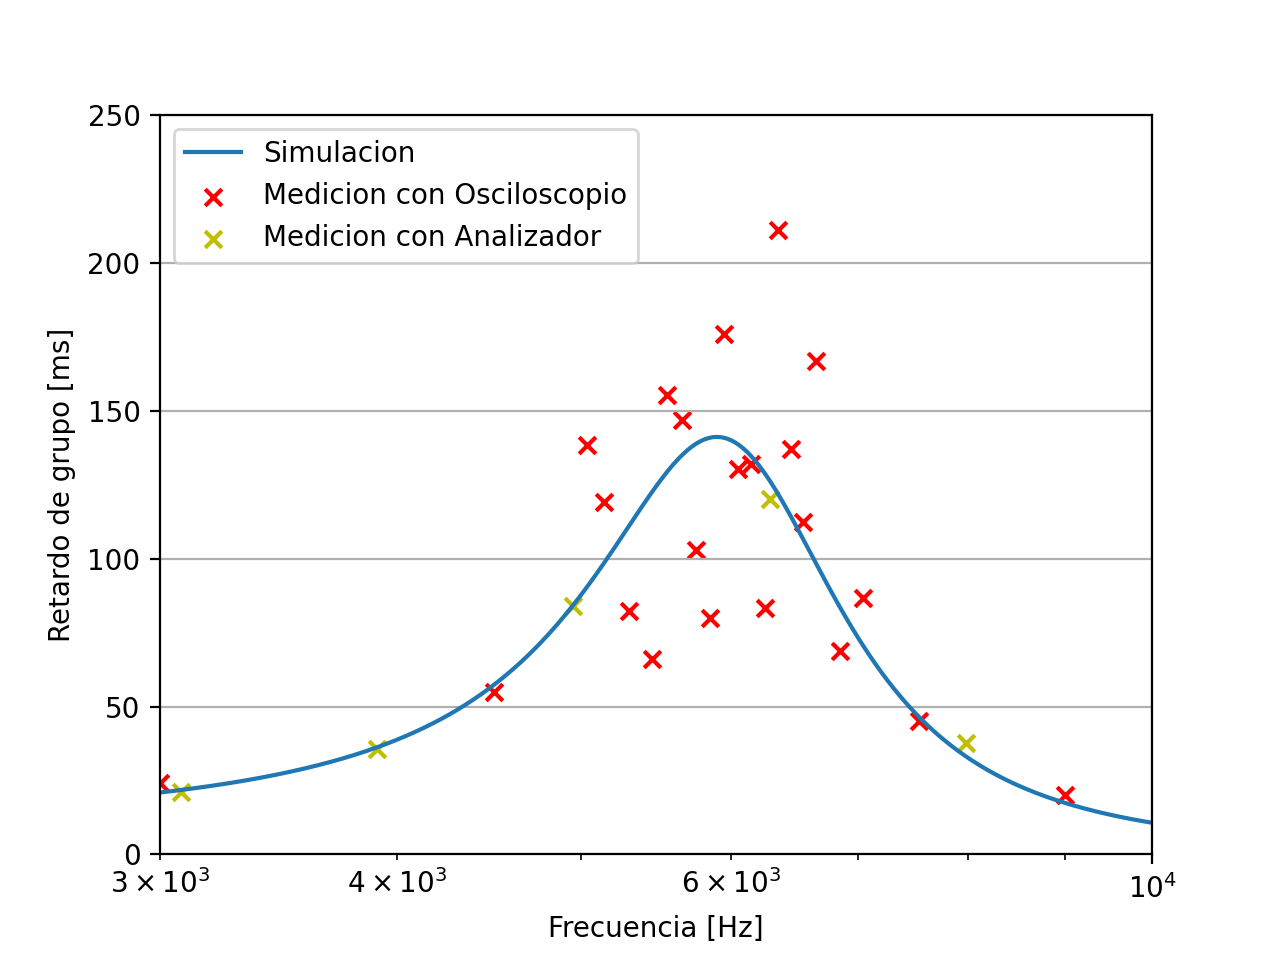
\includegraphics[scale=0.7]{figs/plots/delay_zoom.png}
\caption{Mediciones del retardo de grupo cerca de la banda de paso}
\end{figure}

A diferencia de las mediciones anteriores, la medición del retado de grupo con el osciloscopio no produce valores muy precisos. Sospechamos que esto se debe a demasiado ruido en las mediciones del retardo de fase realizados con los cursores, este ruido no es notable en la respuesta de fase, pero al derivarla el ruido pasa a ser mucho mas significativo.


\chapter{Conclusiones}

Este trabajo practico sirvió para llevar a la practica la teoría moderna de diseños de filtros analógicos. Realizar la implementación física nos ayudó ver cuan bien se traduce la teoría a la practica. Los resultados fueron sorprendentemente positivos, obtuvimos un comportamiento del filtro muy cercano al teórico. Igualmente, vale la pena remarcar de que las limitaciones existen, impuestas sobre todo por comportamientos no ideales de los componentes activos como limites de ancho de banda, rechazo de modo común y slew rate. Y en casos mas extremos, capacitancias e inductancias parásitas y mala adaptación de impedancias pueden llevar a comportamientos no esperados.

La tarea de construir el filtro también nos sirvió para ganar experiencia resolviendo problemas de circuitos de filtrado analógico utilizando instrumentos de laboratorio, ya que inicialmente tuvimos problemas inesperados cuando lo construimos que resultaron ser errores de conexión.

También nos resultó interesante que la datasheet del UAF42 presente formulas convenientes para el diseño del filtro, lo cual es de gran utilidad para alguien que este realizando un filtro pero carezca de los conocimientos necesarios como para hacer el análisis circuital.


\addcontentsline{toc}{chapter}{Referencias}
\printbibliography[title={References}]


\end{document}